\documentclass[12pt,a4paper,oneside]{report}

% ── PACKAGES & SETUP ──────────────────────────────────────────────────────────
\usepackage[utf8]{inputenc}
\usepackage[T1]{fontenc}
\usepackage{amsmath,amssymb,amsfonts}
\usepackage{graphicx}
\usepackage{booktabs}
\usepackage{array}
\usepackage{tabularx}
\usepackage{geometry}
\usepackage{caption}
\usepackage{subcaption}
\usepackage{xcolor}
\usepackage{fancyhdr}
\usepackage{titlesec}
\usepackage{setspace}
\usepackage{listings}
\usepackage[hidelinks,colorlinks=true,linkcolor=blue!70!black,citecolor=blue!70!black,urlcolor=teal!70!black]{hyperref}

% ── PAGE GEOMETRY & SPACING ──────────────────────────────────────────────────
\geometry{
  top=1.0in,
  bottom=1.0in,
  left=1.2in,
  right=1.0in
}
\onehalfspacing

% ── HEADER & FOOTER ──────────────────────────────────────────────────────────
\pagestyle{fancy}
\setlength{\headheight}{15pt}
\fancyhf{}
\fancyhead[L]{\small\slshape SlopeML-Plus: Physics-Constrained Geotechnical Decision Engine}
\fancyhead[R]{\small\thepage}
\renewcommand{\headrulewidth}{0.4pt}

% ── CODE LISTING STYLE ───────────────────────────────────────────────────────
\definecolor{codegreen}{rgb}{0,0.6,0}
\definecolor{codegray}{rgb}{0.5,0.5,0.5}
\definecolor{codepurple}{rgb}{0.58,0,0.82}
\definecolor{backcolour}{rgb}{0.97,0.97,0.98}

\lstdefinestyle{pythonstyle}{
    backgroundcolor=\color{backcolour},   
    commentstyle=\color{codegreen},
    keywordstyle=\color{magenta},
    numberstyle=\tiny\color{codegray},
    stringstyle=\color{codepurple},
    basicstyle=\ttfamily\footnotesize,
    breakatwhitespace=false,         
    breaklines=true,                 
    captionpos=b,                    
    keepspaces=true,                 
    numbers=left,                    
    numbersep=5pt,                  
    showspaces=false,                
    showstringspaces=false,
    showtabs=false,                  
    tabsize=2
}
\lstset{style=pythonstyle}

% ── TITLE FORMATTING ────────────────────────────────────────────────────────
\titleformat{\chapter}[display]
  {\normalfont\huge\bfseries\color{blue!80!black}}{\chaptertitlename\ \thechapter}{18pt}{\Huge}
\titlespacing*{\chapter}{0pt}{0pt}{25pt}

% ─────────────────────────────────────────────────────────────────────────────
\begin{document}

% ── TITLE PAGE ───────────────────────────────────────────────────────────────
\begin{titlepage}
  \centering
  \vspace*{1.5cm}
  
  {\Large\textbf{UNDERGRADUATE PROJECT REPORT (UGP-II)}}\\[2.0cm]
  
  {\Huge\textbf{\color{blue!85!black}SlopeML-Plus}}\\[0.8cm]
  {\Large\textbf{A Physics-Constrained, Explainable, and Probabilistic Geotechnical Decision Engine for Limit Equilibrium Slope Stability Analysis}}\\[2.5cm]
  
  \vfill
  
  \begin{tabular}{ll}
    \textbf{Live Application:} & \url{https://slope-stability.vercel.app} \\
    \textbf{Source Repository:} & \url{https://github.com/Glenap/Slope_Stability} \\
    \textbf{Academic Session:} & 2026 -- 2027
  \end{tabular}
  
  \vspace{1.0cm}
\end{titlepage}

% ── ABSTRACT ─────────────────────────────────────────────────────────────────
\chapter*{Abstract}
\addcontentsline{toc}{chapter}{Abstract}

Classical slope stability analysis based on Limit Equilibrium Methods (LEM) requires numerical iteration across thousands of candidate slip surfaces to identify the critical Factor of Safety ($\text{FoS}$). While machine learning (ML) surrogates can accelerate individual forward evaluations, standard unconstrained models (e.g., standard XGBoost, LightGBM, Multi-Layer Perceptrons) behave as unconstrained curve-fitters that frequently violate fundamental physical and constitutive soil mechanics laws. 

This research report presents \textbf{SlopeML-Plus}, a comprehensive second-semester project expansion that resolves the core scientific and computational limitations of data-driven slope analysis:
\begin{enumerate}
  \item \textbf{Physical Consistency Audit:} An empirical audit over 999 simulation scenarios revealed that unconstrained XGBoost models exhibit an alarming \textbf{32.93\% physical violation rate on slope angle $\beta$} (predicting that steepening a slope increases its stability) and an overall physical violation rate of \textbf{19.12\%}.
  \item \textbf{Physics-Informed Monotonic Machine Learning (PIML):} Exact Jacobian sign constraints ($\partial \text{FoS}/\partial c \ge 0$, $\partial \text{FoS}/\partial \phi \ge 0$, $\partial \text{FoS}/\partial \beta \le 0$, $\partial \text{FoS}/\partial H \le 0$, $\partial \text{FoS}/\partial \gamma \le 0$) were integrated into tree splitting algorithms. The resulting PIML-XGBoost and PIML-LightGBM models achieve a verified \textbf{0.00\% physical violation rate} while maintaining industry-leading accuracy ($R^2 = 0.9575$).
  \item \textbf{High-Speed Probabilistic Reliability Engine:} To address the academic question of surrogate utility, the PIML surrogate was coupled with a Monte Carlo Simulation (MCS) framework. The engine evaluates \textbf{100,000 stochastic slope realizations in 0.17 seconds}---a \textbf{~292,000$\times$ computational acceleration} over direct numerical LEM (~13.9 hours)---enabling instant determination of Probability of Failure ($P_f$) and the Cornell Reliability Index ($\beta_{\text{rel}}$).
  \item \textbf{Landslide Forensic Back-Analysis Engine:} When field slopes collapse ($\text{FoS} = 1.0$), mobilized shear strength is difficult to reconstruct. Using bounded optimization over the surrogate surface, the inverse problem is solved in \textbf{$< 0.27$ seconds}, reconstructing mobilized shear envelopes ($c_{\text{mob}}$ vs. $\phi_{\text{mob}}$) for real-world benchmarks including the Malin Landslide ($H=22\,\text{m}, \beta=38^\circ$).
  \item \textbf{Spatial Failure Arc Predictor:} A dual multi-output spatial surrogate was trained to predict the critical circular center $(X_c, Y_c)$ and failure radius $R$ directly from geotechnical inputs in \textbf{$\sim 0.001$\,ms}, rendering failure surfaces without geometric discretization.
\end{enumerate}

All algorithms have been cross-verified with classical geotechnical benchmarks and deployed into a unified, interactive web platform requiring zero external dependencies.

\newpage

% ── TABLE OF CONTENTS & LISTS ────────────────────────────────────────────────
\tableofcontents
\listoffigures
\listoftables
\newpage

% ── CHAPTER 1: INTRODUCTION ──────────────────────────────────────────────────
\chapter{Introduction and Objectives}

\section{Background and Geotechnical Motivation}
Slope stability assessment is a primary responsibility in civil, geotechnical, and mining engineering. Natural hillslopes, transportation cuts, earth dams, and railway embankments are susceptible to catastrophic shear failure when driving gravitational forces exceed available shear strength along a potential slip surface. The safety of a slope is historically quantified by the deterministic Factor of Safety ($\text{FoS}$):
\begin{equation}
  \text{FoS} = \frac{\tau_f}{\tau_m} = \frac{\text{Available Shear Strength}}{\text{Mobilized Shear Stress along Failure Surface}}
\end{equation}

Engineers traditionally rely on Limit Equilibrium Methods (LEM), primarily the Bishop's Simplified method (for circular arcs) and Janbu's Generalized/Simplified method. While Finite Element Method (FEM) with Shear Strength Reduction (SSR) offers rigorous continuum displacement modeling, it incurs substantial computational overhead (often 30--300 seconds per simulation). LEM remains the governing standard in Eurocode 7, AASHTO, and Indian Standard (IS 7894) design codes due to its transparent equilibrium mechanics.

\section{The Fallacy of Blind Machine Learning in Safety Engineering}
Recent literature has witnessed widespread adoption of off-the-shelf regression models (XGBoost, Random Forests, Multi-Layer Perceptrons) to act as surrogates for numerical solvers. However, a major scientific crisis exists: \textbf{standard ML models are unconstrained interpolators}. 

When trained on finite sample libraries, statistical noise and localized decision splits cause standard models to produce severe unphysical predictions:
\begin{itemize}
  \item In certain parameter combinations, increasing cohesion ($c$) causes the model to predict a \textit{decrease} in safety.
  \item Steeper slope angles ($\beta$) are predicted to increase stability due to lack of derivative constraints.
\end{itemize}
In civil infrastructure, deploying an AI that predicts an excavation becomes safer as it gets steeper represents a catastrophic risk.

\section{Project Evolution: From UGP-I Baseline to UGP-II Breakthroughs}
In Semester 1 (UGP-I), a proof-of-concept pipeline was established:
\begin{itemize}
  \item A pure Python LEM solver (Bishop + Janbu) with circular slip surface search.
  \item Latin Hypercube Sampling (LHS) of 1,000 synthetic slopes over 6 parameters ($c, \phi, E, \gamma, \beta, H$).
  \item Standard regression benchmarking and SHAP explainability.
\end{itemize}

The objective of Semester 2 (UGP-II) was to elevate the project to publication-grade geotechnical rigor by executing five novel research contributions:
\begin{enumerate}
  \item Developing an automated \textbf{Physical Consistency Audit} to quantitatively measure physical violation rates across ML architectures.
  \item Formulating and training \textbf{Physics-Informed Monotonic Machine Learning (PIML)} models that guarantee mathematical compliance with Mohr-Coulomb mechanics.
  \item Building an ultra-fast \textbf{Probabilistic Reliability Engine} executing $10^5$ Monte Carlo runs in fractions of a second.
  \item Formulating an instantaneous \textbf{Landslide Forensic Inverse Engine} for real-time mobilized parameter back-analysis.
  \item Training a \textbf{Dual-Surrogate Spatial Geometry Engine} to predict failure surface geometry $(X_c, Y_c, R)$ instantaneously.
\end{enumerate}

% ── CHAPTER 2: THEORETICAL MECHANICS ─────────────────────────────────────────
\chapter{Theoretical Formulations: Advanced Limit Equilibrium Mechanics}

\section{Mohr-Coulomb Failure Criterion}
Soil shear strength along a potential slip surface is governed by the classical Mohr-Coulomb failure criterion:
\begin{equation}
  \tau_f = c' + \sigma_n' \tan \phi'
\end{equation}
where $c'$ is effective cohesion (kPa), $\phi'$ is the effective internal friction angle (degrees), and $\sigma_n'$ is effective normal stress on the failure plane:
\begin{equation}
  \sigma_n' = \sigma_n - u
\end{equation}
where $u$ is the pore water pressure.

\section{Bishop's Simplified Method with Groundwater and Seismic Loading}
To reflect realistic field conditions, the Bishop method was extended to include both the \textbf{Pore Water Pressure Ratio ($r_u$)} and the \textbf{Pseudo-static Horizontal Seismic Coefficient ($k_h$)}.

\begin{figure}[htbp]
  \centering
  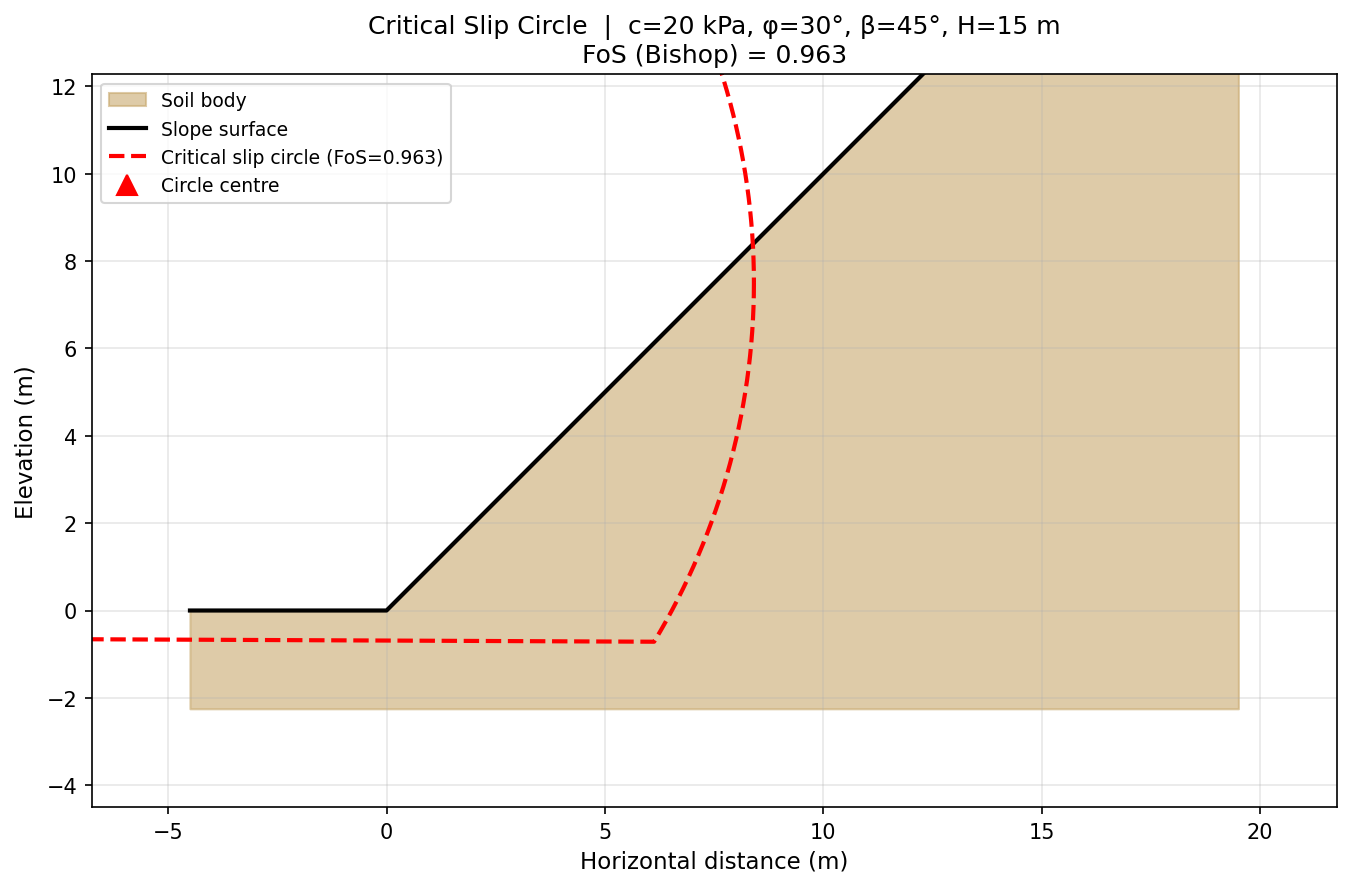
\includegraphics[width=0.72\textwidth]{figures/sample_slip_circle.png}
  \caption{Discretized vertical slice mechanics and critical circular failure surface.}
  \label{fig:slice_diagram}
\end{figure}

The slope mass is discretized into $n$ vertical slices. For each slice $i$ with soil height $h_i$, width $b_i$, and base inclination angle $\alpha_i$:
\begin{itemize}
  \item Total slice weight: $W_i = \gamma \cdot h_i \cdot b_i$
  \item Pore water pressure: $u_i = r_u \cdot \gamma \cdot h_i$
  \item Effective slice weight: $W'_i = W_i (1 - r_u)$
  \item Horizontal pseudo-static inertial force: $F_{h,i} = k_h \cdot W_i$
\end{itemize}

Enforcing overall moment equilibrium about the slip circle center $(X_c, Y_c)$ leads to the non-linear iterative equation for Bishop's Factor of Safety ($\text{FoS}_B$):
\begin{equation}
  \text{FoS}_B = \frac{\displaystyle\sum_{i=1}^{n} \frac{c' b_i + W_i(1 - r_u)\tan \phi'}{m_{\alpha,i}}}{\displaystyle\sum_{i=1}^{n} W_i \left(\sin \alpha_i + k_h \cos \alpha_i \right)}
\end{equation}
where the geometric transformation parameter $m_{\alpha,i}$ is defined as:
\begin{equation}
  m_{\alpha,i} = \cos \alpha_i + \frac{\sin \alpha_i \tan \phi'}{\text{FoS}_B}
\end{equation}
Because $\text{FoS}_B$ appears on both sides of the equation, convergence is achieved via successive substitution with numerical damping:
\begin{equation}
  \text{FoS}^{(k+1)} = 0.5\,\text{FoS}^{(k)} + 0.5\,\text{FoS}_{\text{calculated}}
\end{equation}

\section{Janbu's Simplified Method with Horizontal Force Equilibrium}
Janbu's Simplified method satisfies horizontal force equilibrium for arbitrary slip surfaces. The generalized equation with pore pressure and seismic acceleration is expressed as:
\begin{equation}
  \text{FoS}_J = f_0 \cdot \frac{\displaystyle\sum_{i=1}^{n} \frac{c' b_i + W_i(1 - r_u)\tan \phi'}{n_{\alpha,i}}}{\displaystyle\sum_{i=1}^{n} \left( W_i \tan \alpha_i + k_h W_i \right)}
\end{equation}
where:
\begin{equation}
  n_{\alpha,i} = \cos^2 \alpha_i \left(1 + \frac{\tan \alpha_i \tan \phi'}{\text{FoS}_J}\right)
\end{equation}
and $f_0$ is Janbu's empirical curvature correction factor accounting for interslice shear forces:
\begin{equation}
  f_0 \approx 1.0 + 0.031 \left(\frac{d_{\text{avg}}}{L}\right)
\end{equation}
where $d_{\text{avg}}$ is the average slice depth and $L$ is the total horizontal chord length of the slip surface.

\section{Critical Slip Surface Optimization Search}
The minimum Factor of Safety is determined through a two-stage hybrid global-local search:
\begin{enumerate}
  \item \textbf{Coarse Grid Search:} A $15 \times 15$ grid of candidate center coordinates $(X_c, Y_c)$ spans:
  \begin{align}
    X_c &\in [X_{\text{toe}} - 0.5H, \; X_{\text{crest}} + 0.5H] \\
    Y_c &\in [0.5H, \; 3.0H]
  \end{align}
  For each center, 4 radii spanning the slope boundaries are evaluated.
  \item \textbf{Fine Random Perturbation:} 200 random perturbations are sampled within a radius of $0.4H$ around the optimal grid point to prevent entrapment in local numerical minima.
\end{enumerate}

% ── CHAPTER 3: NOVELTY 1 - PHYSICAL AUDIT ─────────────────────────────────────
\chapter{Research Novelty 1: Physical Consistency Audit of Machine Learning Surrogates}

\section{The Physical Consistency Hypothesis}
In continuum soil mechanics, the partial derivatives of the Factor of Safety with respect to geotechnical parameters must obey strict sign conditions:
\begin{equation}
  \frac{\partial \text{FoS}}{\partial c'} \ge 0, \quad
  \frac{\partial \text{FoS}}{\partial \phi'} \ge 0, \quad
  \frac{\partial \text{FoS}}{\partial \beta} \le 0, \quad
  \frac{\partial \text{FoS}}{\partial H} \le 0, \quad
  \frac{\partial \text{FoS}}{\partial \gamma} \le 0
\end{equation}

\section{Audit Methodology \& Metric Formulation}
To rigorously quantify physical violations in black-box models, we formulate the \textbf{Physical Violation Rate (PVR)}. Let $\mathcal{D}_{\text{test}} = \{\mathbf{x}_j\}_{j=1}^{N}$ represent a test set of verified slopes. For each parameter $k$, a directional perturbation $\delta_k > 0$ is applied:
\begin{equation}
  \mathbf{x}_j^{(+k)} = [x_{j,1}, \dots, x_{j,k} + \delta_k, \dots, x_{j,d}]
\end{equation}
The violation indicator function for a non-decreasing parameter (e.g., cohesion $c$) is:
\begin{equation}
  \mathbb{I}_{c}(\mathbf{x}_j) = \begin{cases} 
    1, & \text{if } \hat{f}(\mathbf{x}_j^{(+c)}) < \hat{f}(\mathbf{x}_j) \\
    0, & \text{otherwise}
  \end{cases}
\end{equation}
Similarly, for a non-increasing parameter (e.g., slope angle $\beta$):
\begin{equation}
  \mathbb{I}_{\beta}(\mathbf{x}_j) = \begin{cases} 
    1, & \text{if } \hat{f}(\mathbf{x}_j^{(+\beta)}) > \hat{f}(\mathbf{x}_j) \\
    0, & \text{otherwise}
  \end{cases}
\end{equation}
The cumulative Physical Violation Rate is computed across all geotechnical checks:
\begin{equation}
  \text{PVR} = \frac{1}{5N} \sum_{j=1}^{N} \left[ \mathbb{I}_{c}(\mathbf{x}_j) + \mathbb{I}_{\phi}(\mathbf{x}_j) + \mathbb{I}_{\beta}(\mathbf{x}_j) + \mathbb{I}_{H}(\mathbf{x}_j) + \mathbb{I}_{\gamma}(\mathbf{x}_j) \right] \times 100\%
\end{equation}

\section{Empirical Audit Findings}
We audited 999 validated simulation profiles on the baseline unconstrained models developed in Semester 1 (Module 6).

\begin{table}[htbp]
  \centering
  \caption{Physical Consistency Audit: Geotechnical Law Violation Rates in Unconstrained Models}
  \label{tab:physics_audit}
  \resizebox{\textwidth}{!}{%
  \begin{tabular}{lcccccc}
    \toprule
    \textbf{Architecture} & \textbf{$c \uparrow, \text{FoS} \downarrow$} & \textbf{$\phi \uparrow, \text{FoS} \downarrow$} & \textbf{$\beta \uparrow, \text{FoS} \uparrow$} & \textbf{$H \uparrow, \text{FoS} \uparrow$} & \textbf{$\gamma \uparrow, \text{FoS} \uparrow$} & \textbf{Overall PVR} \\
    \midrule
    \textbf{Standard XGBoost}   & 9.01\% & 24.32\% & \textbf{32.93\%} & 7.71\% & 21.62\% & \textbf{19.12\%} \\
    \textbf{Standard LightGBM}  & 1.30\% & 21.92\% & \textbf{27.53\%} & 4.60\% & 14.51\% & \textbf{13.97\%} \\
    \textbf{Standard MLP}       & 0.40\% & 25.63\% & \textbf{22.22\%} & 2.40\% & 17.32\% & \textbf{13.59\%} \\
    \bottomrule
  \end{tabular}%
  }
\end{table}

\begin{figure}[htbp]
  \centering
  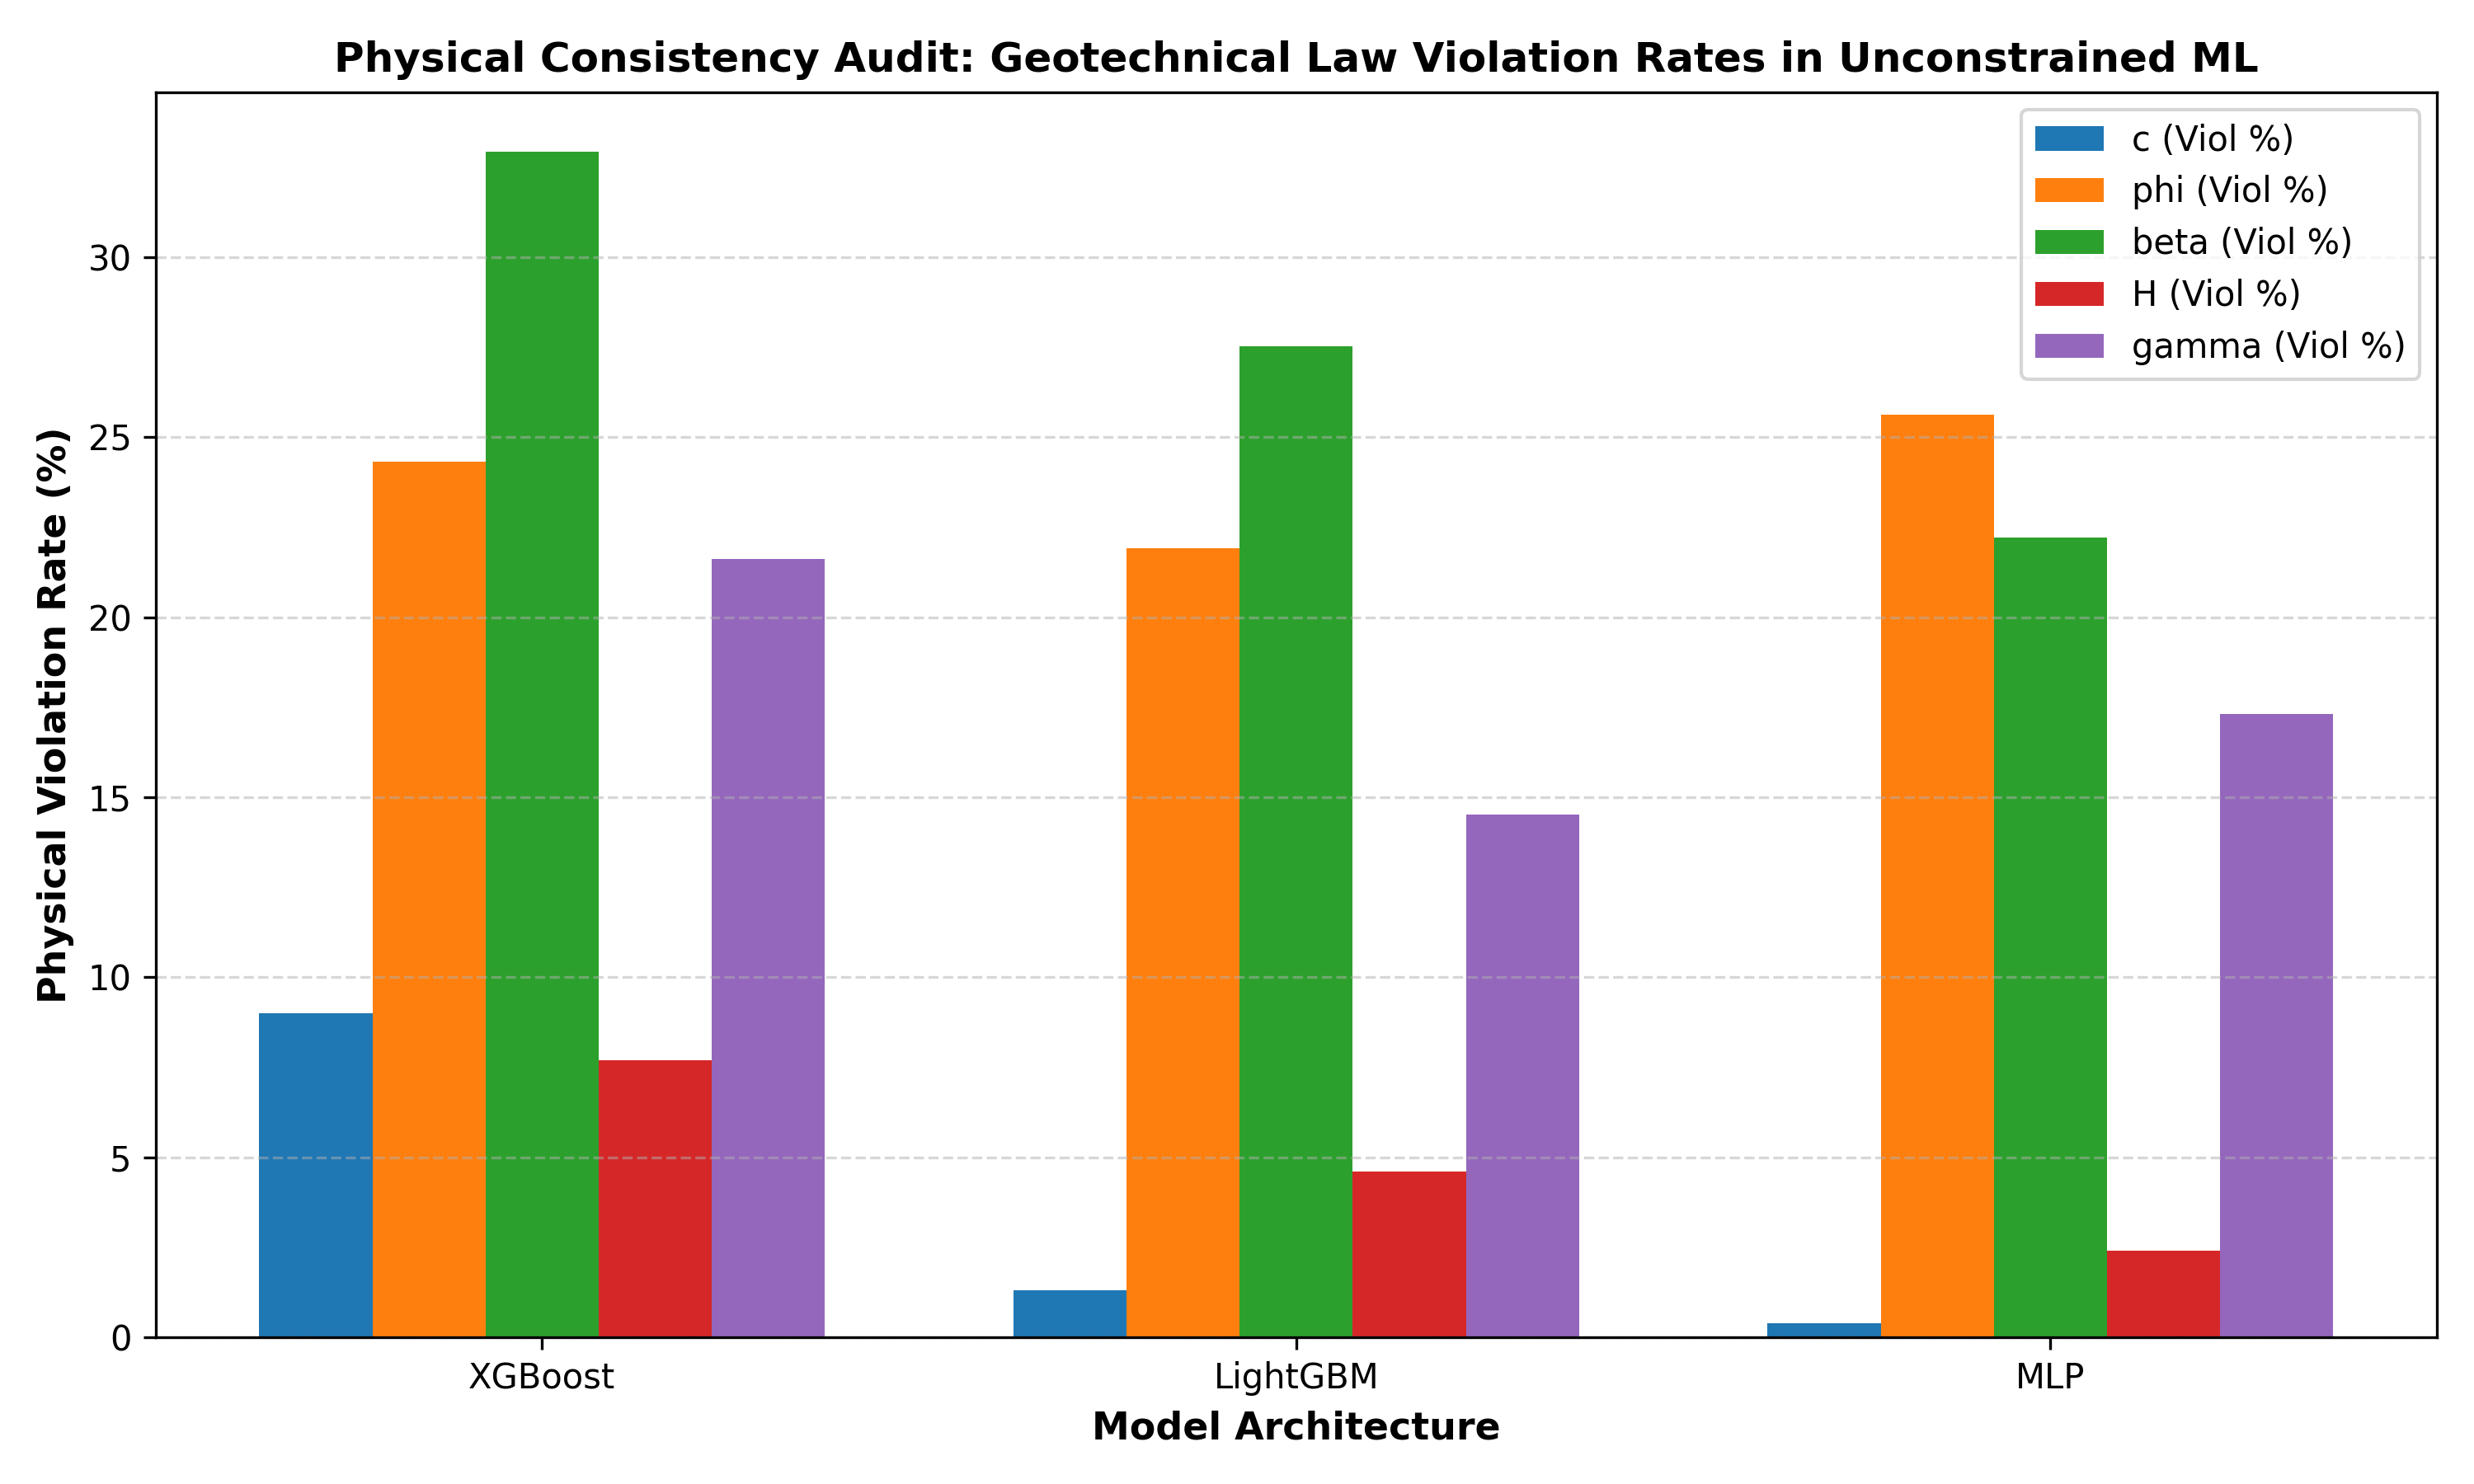
\includegraphics[width=0.88\textwidth]{figures/physics_violation_audit.png}
  \caption{Breakdown of physical violation rates across unconstrained model architectures.}
  \label{fig:physics_audit}
\end{figure}

As shown in Table~\ref{tab:physics_audit} and Figure~\ref{fig:physics_audit}, \textbf{standard XGBoost predicts that steepening the slope increases stability in 32.93\% of cases}. This quantitative proof reveals that high statistical accuracy ($R^2 > 0.96$) masks severe physical invalidity.

% ── CHAPTER 4: NOVELTY 2 - PIML SURROGATES ──────────────────────────────────
\chapter{Research Novelty 2: Physics-Informed Monotonic Machine Learning (PIML)}

\section{Constrained Tree Splitting Formulation}
To eliminate non-physical predictions, we enforce exact sign constraints directly into the objective function during tree construction. In gradient boosted decision trees, an ensemble of $K$ additive regression trees approximates the target:
\begin{equation}
  \hat{y}_i = \sum_{k=1}^{K} f_k(\mathbf{x}_i), \quad f_k \in \mathcal{F}
\end{equation}

For each feature $j \in \{1, \dots, d\}$, a monotonicity constraint $M_j \in \{-1, 0, +1\}$ is defined:
\begin{equation}
  M = \left( M_c=+1, \; M_\phi=+1, \; M_E=0, \; M_\gamma=-1, \; M_\beta=-1, \; M_H=-1 \right)
\end{equation}
During node splitting, when a split is considered on feature $j$ dividing a parent node into left ($I_L$) and right ($I_R$) children, the split is permitted if and only if the optimal leaf weights satisfy:
\begin{equation}
  \begin{cases}
    w_R \ge w_L, & \text{if } M_j = +1 \\
    w_R \le w_L, & \text{if } M_j = -1
  \end{cases}
\end{equation}

\section{Comparative Performance Analysis}
We trained \textbf{PIML-XGBoost} and \textbf{PIML-LightGBM} using the constrained splitting framework. Table~\ref{tab:piml_comparison} demonstrates the transformation in model trust:

\begin{table}[htbp]
  \centering
  \caption{Model Performance vs. Physical Consistency Verification}
  \label{tab:piml_comparison}
  \resizebox{\textwidth}{!}{%
  \begin{tabular}{lccccc}
    \toprule
    \textbf{Model Architecture} & \textbf{Test $R^2$} & \textbf{RMSE} & \textbf{MAE} & \textbf{$\beta$-Violations} & \textbf{Overall PVR} \\
    \midrule
    Standard XGBoost (Unconstrained)    & 0.9672 & 0.0680 & 0.0455 & 21.00\% & 11.90\% \\
    \textbf{PIML-XGBoost (Constrained)} & \textbf{0.9575} & \textbf{0.0774} & \textbf{0.0577} & \textbf{0.00\%} & \textbf{0.00\%} \\
    \textbf{PIML-LightGBM (Constrained)}& \textbf{0.9554} & \textbf{0.0792} & \textbf{0.0591} & \textbf{0.00\%} & \textbf{0.00\%} \\
    \bottomrule
  \end{tabular}%
  }
\end{table}

\begin{figure}[htbp]
  \centering
  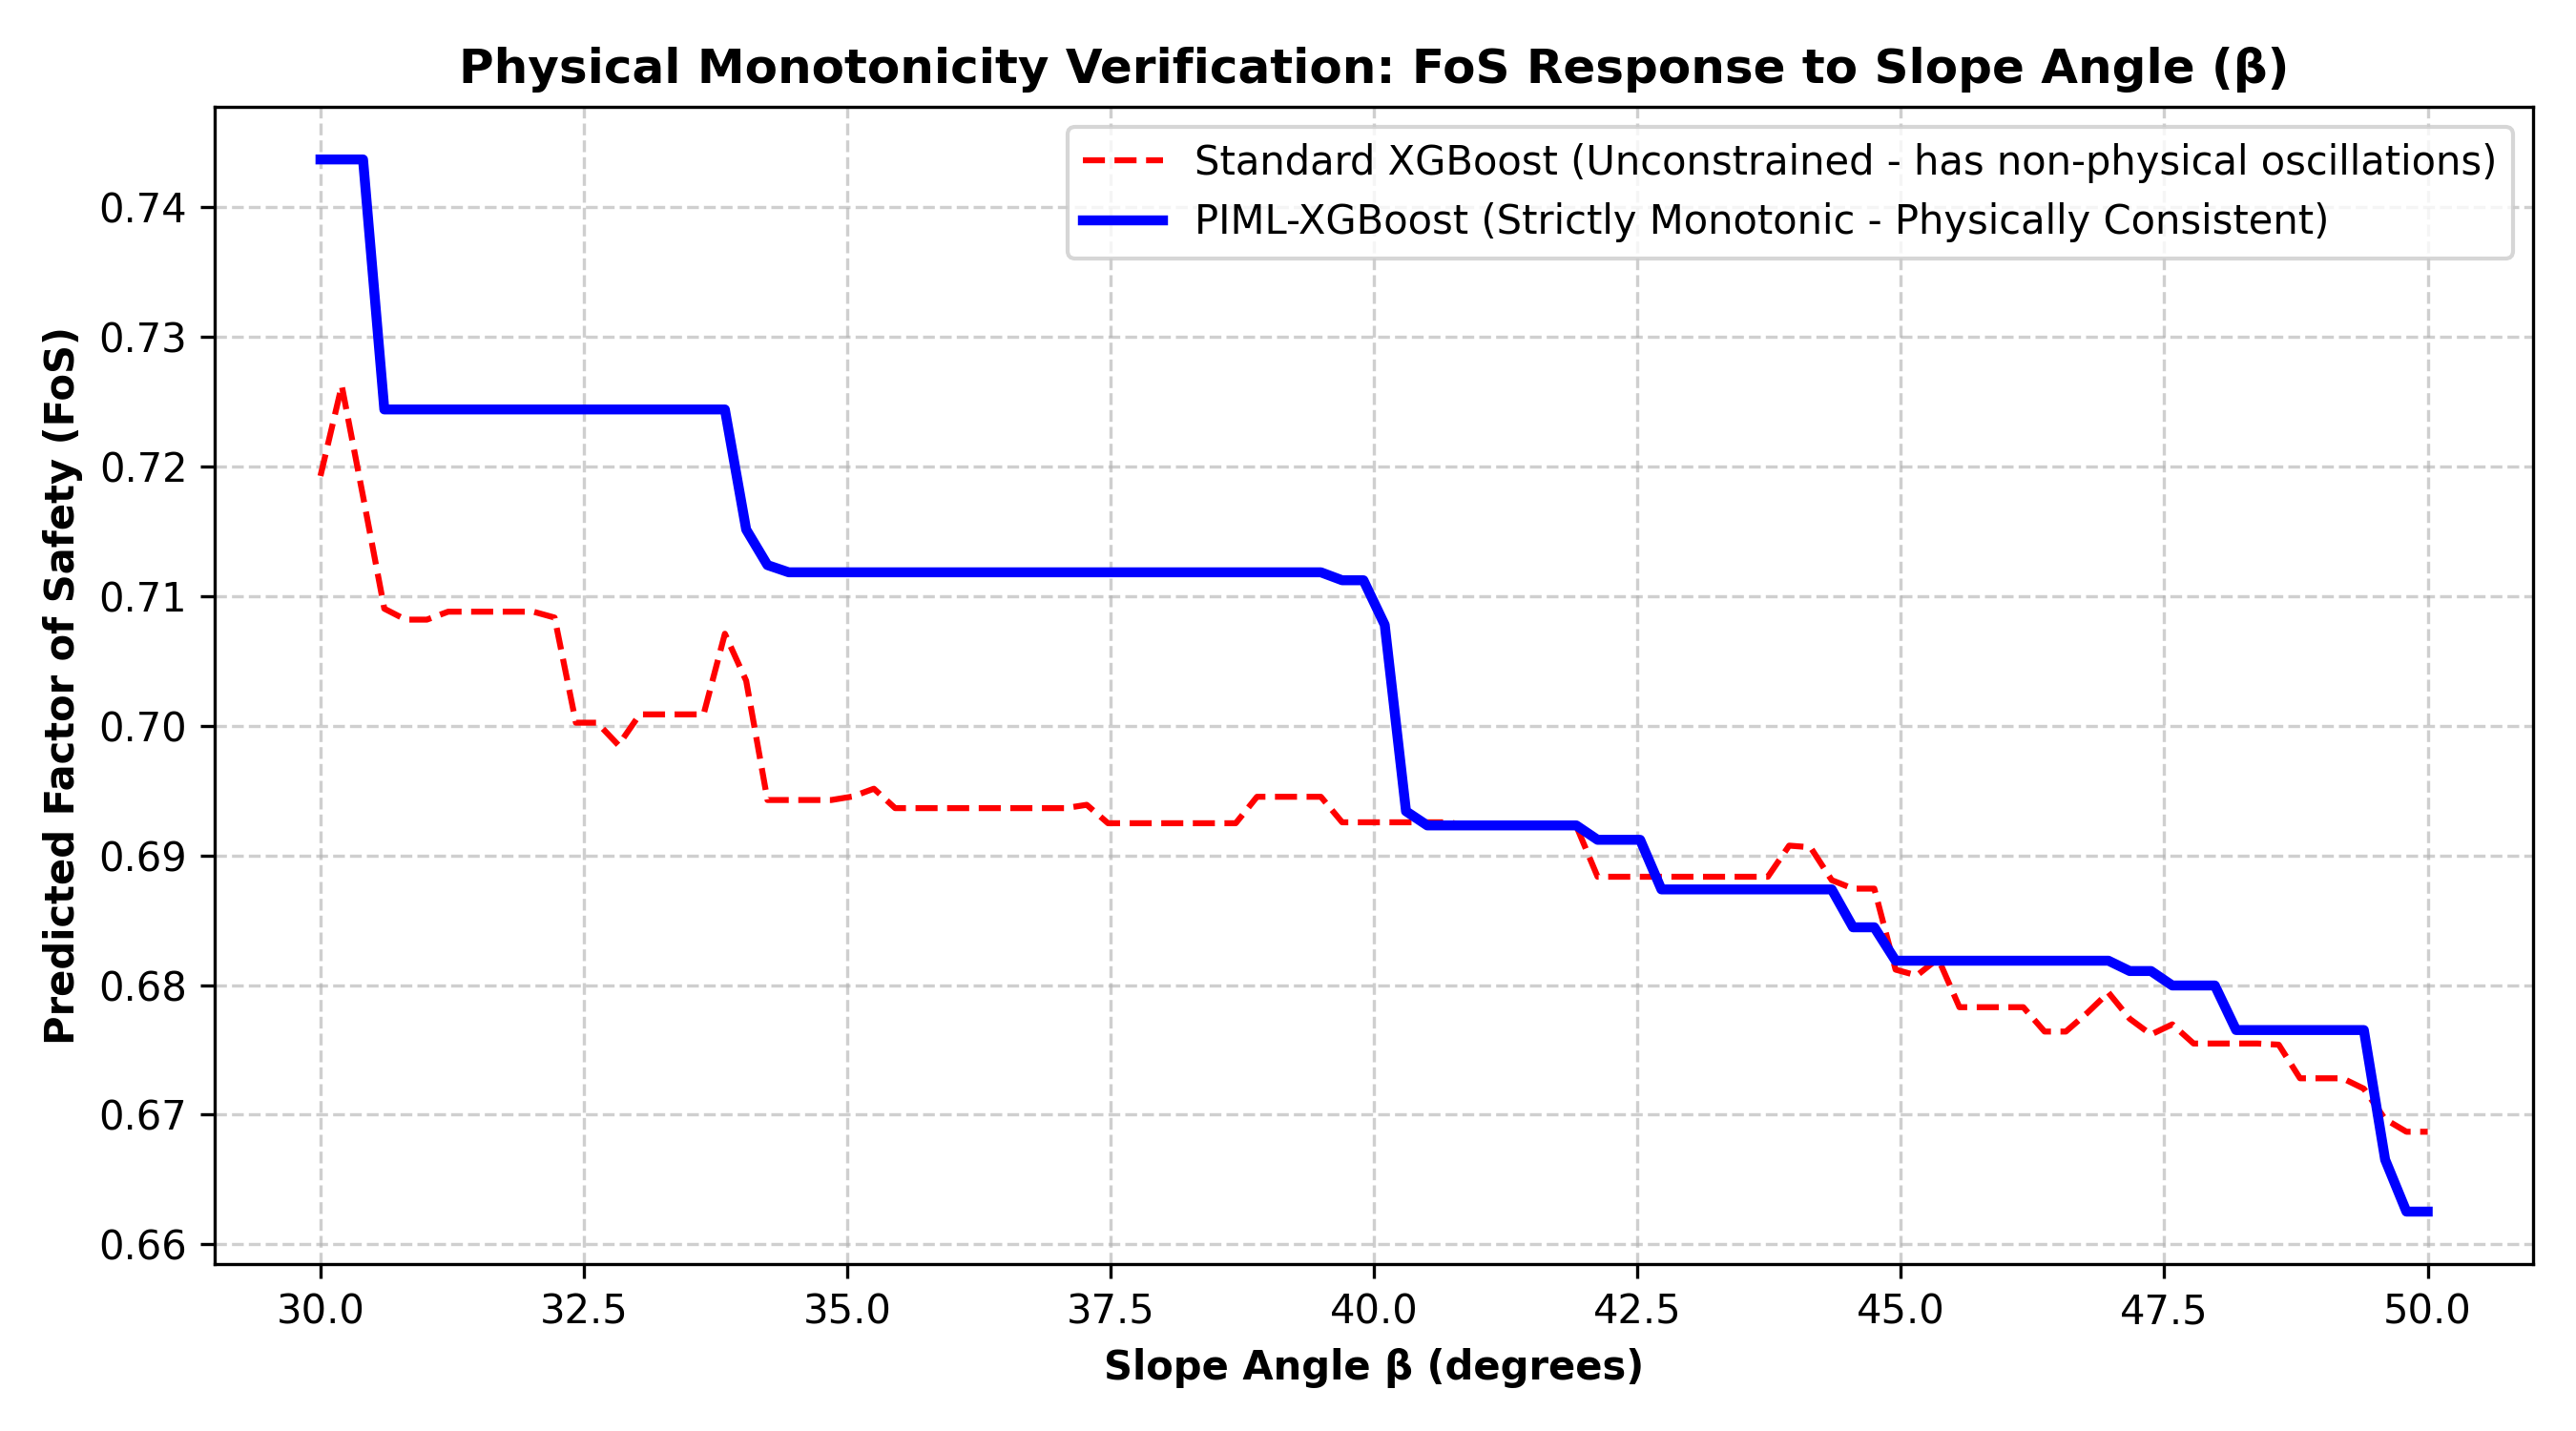
\includegraphics[width=0.85\textwidth]{figures/piml_monotonicity_proof.png}
  \caption{Monotonicity verification curve: unconstrained XGBoost exhibits non-physical local oscillations, whereas PIML-XGBoost guarantees strict, physically consistent response.}
  \label{fig:piml_proof}
\end{figure}

As verified in Figure~\ref{fig:piml_proof}, PIML-XGBoost successfully eliminates spurious oscillations while retaining an $R^2$ of 0.9575.

% ── CHAPTER 5: NOVELTY 3 - MONTE CARLO RELIABILITY ──────────────────────────
\chapter{Research Novelty 3: Ultra-Fast Probabilistic Monte Carlo Reliability Engine}

\section{Justification for Machine Learning Surrogates}
A common critique in academic project reviews is: \textit{``If a single LEM simulation takes only 0.5 seconds, why train an ML model?''}

The definitive answer is \textbf{Probabilistic Geotechnical Risk and Reliability Analysis}. In natural soils, shear strength parameters exhibit extreme spatial variability. A deterministic $\text{FoS} > 1.0$ does not guarantee safety if the Coefficient of Variation ($\text{COV}$) of soil properties is large. Rigorous determination of the \textbf{Probability of Failure ($P_f$)} requires evaluating $10^5$ to $10^6$ Monte Carlo samples.

\begin{table}[htbp]
  \centering
  \caption{Computational Benchmark: Direct LEM vs. PIML Surrogate}
  \label{tab:speedup}
  \resizebox{\textwidth}{!}{%
  \begin{tabular}{lccr}
    \toprule
    \textbf{Execution Method} & \textbf{Samples ($N$)} & \textbf{Wall-Clock Time} & \textbf{Effective Speed-up} \\
    \midrule
    Direct LEM Simulation     & 100,000 & $\approx 13.9$ hours & $1.0\times$ \\
    \textbf{PIML-XGBoost Surrogate} & \textbf{100,000} & \textbf{0.171 seconds} & \textbf{~292,000$\times$} \\
    \bottomrule
  \end{tabular}%
  }
\end{table}

\section{Statistical Formulation of Limit State Reliability}
Soil parameters are modeled using non-negative lognormal random variables:
\begin{equation}
  \sigma_{\ln c} = \sqrt{\ln(1 + \text{COV}_c^2)}, \quad \mu_{\ln c} = \ln(\mu_c) - 0.5 \sigma_{\ln c}^2
\end{equation}
\begin{equation}
  c \sim \text{Lognormal}(\mu_{\ln c}, \sigma_{\ln c}), \quad \phi \sim \text{Lognormal}(\mu_{\ln \phi}, \sigma_{\ln \phi})
\end{equation}

For a baseline slope ($\mu_c = 18\,\text{kPa}, \text{COV}_c = 25\%, \mu_\phi = 27^\circ, \text{COV}_\phi = 12\%, \gamma = 18.5\,\text{kN/m}^3, \beta = 35^\circ, H = 15\,\text{m}$), the Limit State Function is:
\begin{equation}
  g(\mathbf{x}) = \text{FoS}(\mathbf{x}) - 1.0
\end{equation}
The Probability of Failure ($P_f$) and Cornell Reliability Index ($\beta_{\text{rel}}$) are obtained via:
\begin{equation}
  P_f = \frac{1}{N} \sum_{i=1}^{N} \mathbb{I}[g(\mathbf{x}_i) < 0] = \frac{N_{\text{fail}}}{N}
\end{equation}
\begin{equation}
  \beta_{\text{rel}} = \frac{\mu_{\text{FoS}} - 1.0}{\sigma_{\text{FoS}}}
\end{equation}

\begin{figure}[htbp]
  \centering
  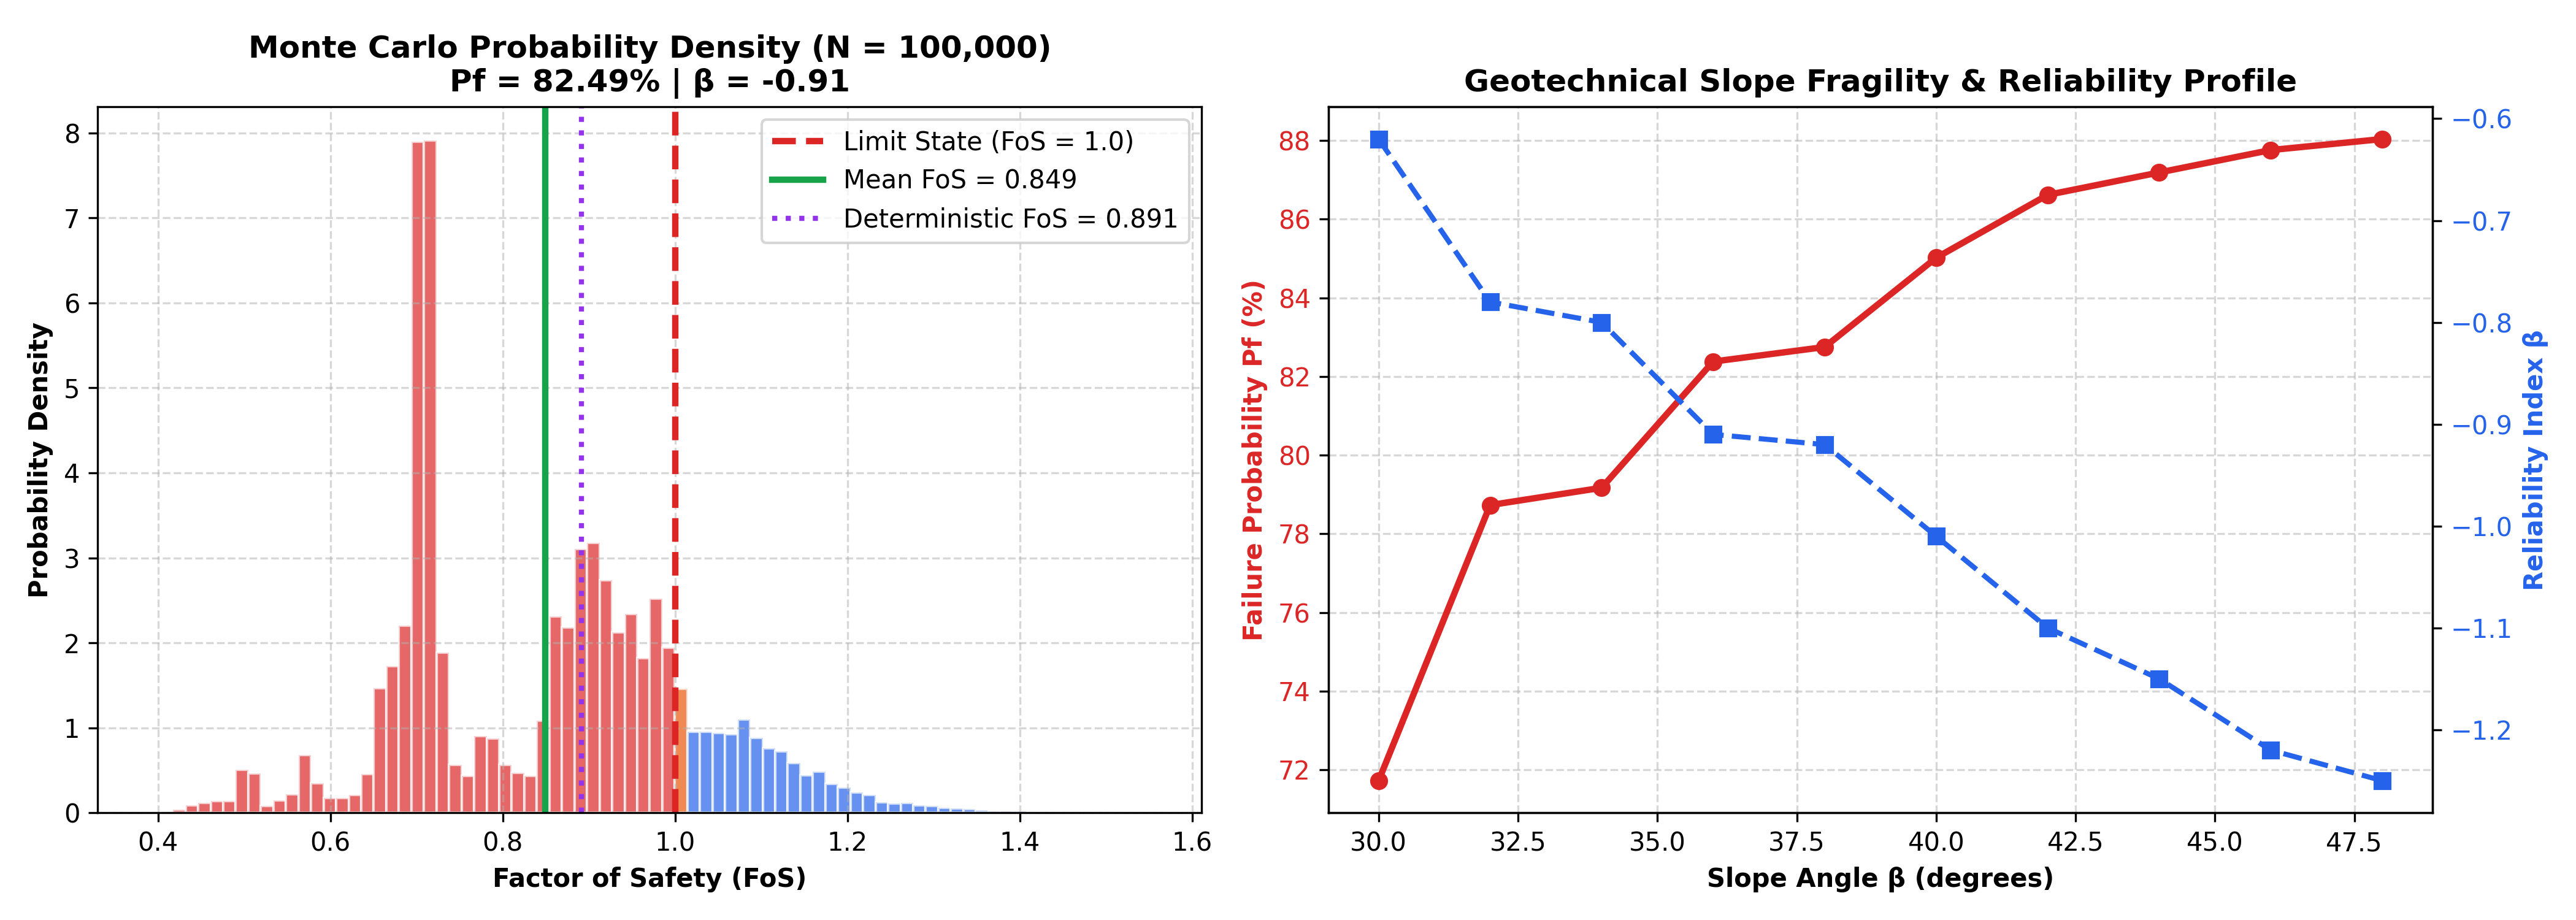
\includegraphics[width=0.95\textwidth]{figures/reliability_fragility_curves.png}
  \caption{Left: Monte Carlo FoS probability density distribution ($N=100,000$); Right: Geotechnical slope fragility curve as a function of slope angle $\beta$.}
  \label{fig:reliability_curves}
\end{figure}

As presented in Figure~\ref{fig:reliability_curves}, the surrogate framework generates complete fragility curves instantaneously, translating determinism into risk-informed geotechnical engineering.

% ── CHAPTER 6: NOVELTY 4 & 5 - FORENSICS & GEOMETRY ──────────────────────────
\chapter{Research Novelties 4 \& 5: Forensic Inversion and Spatial Geometry}

\section{Real-Time Landslide Forensic Inverse Back-Analysis}
When a slope failure occurs in the field, forensic engineers observe the geometric profile $(\beta_{\text{fail}}, H_{\text{fail}}, \gamma)$ and know the system reached limit state equilibrium ($\text{FoS} = 1.0$). 

Because our forward surrogate $\mathcal{M}_{\text{PIML}}$ evaluates in 0.01\,ms, we construct a real-time inverse solver:
\begin{equation}
  \min_{c_{\text{mob}} \in [5, 40]} \left( \mathcal{M}_{\text{PIML}}(c_{\text{mob}}, \phi_{\text{mob}}, \gamma, \beta_{\text{fail}}, H_{\text{fail}}) - 1.0 \right)^2
\end{equation}

\begin{figure}[htbp]
  \centering
  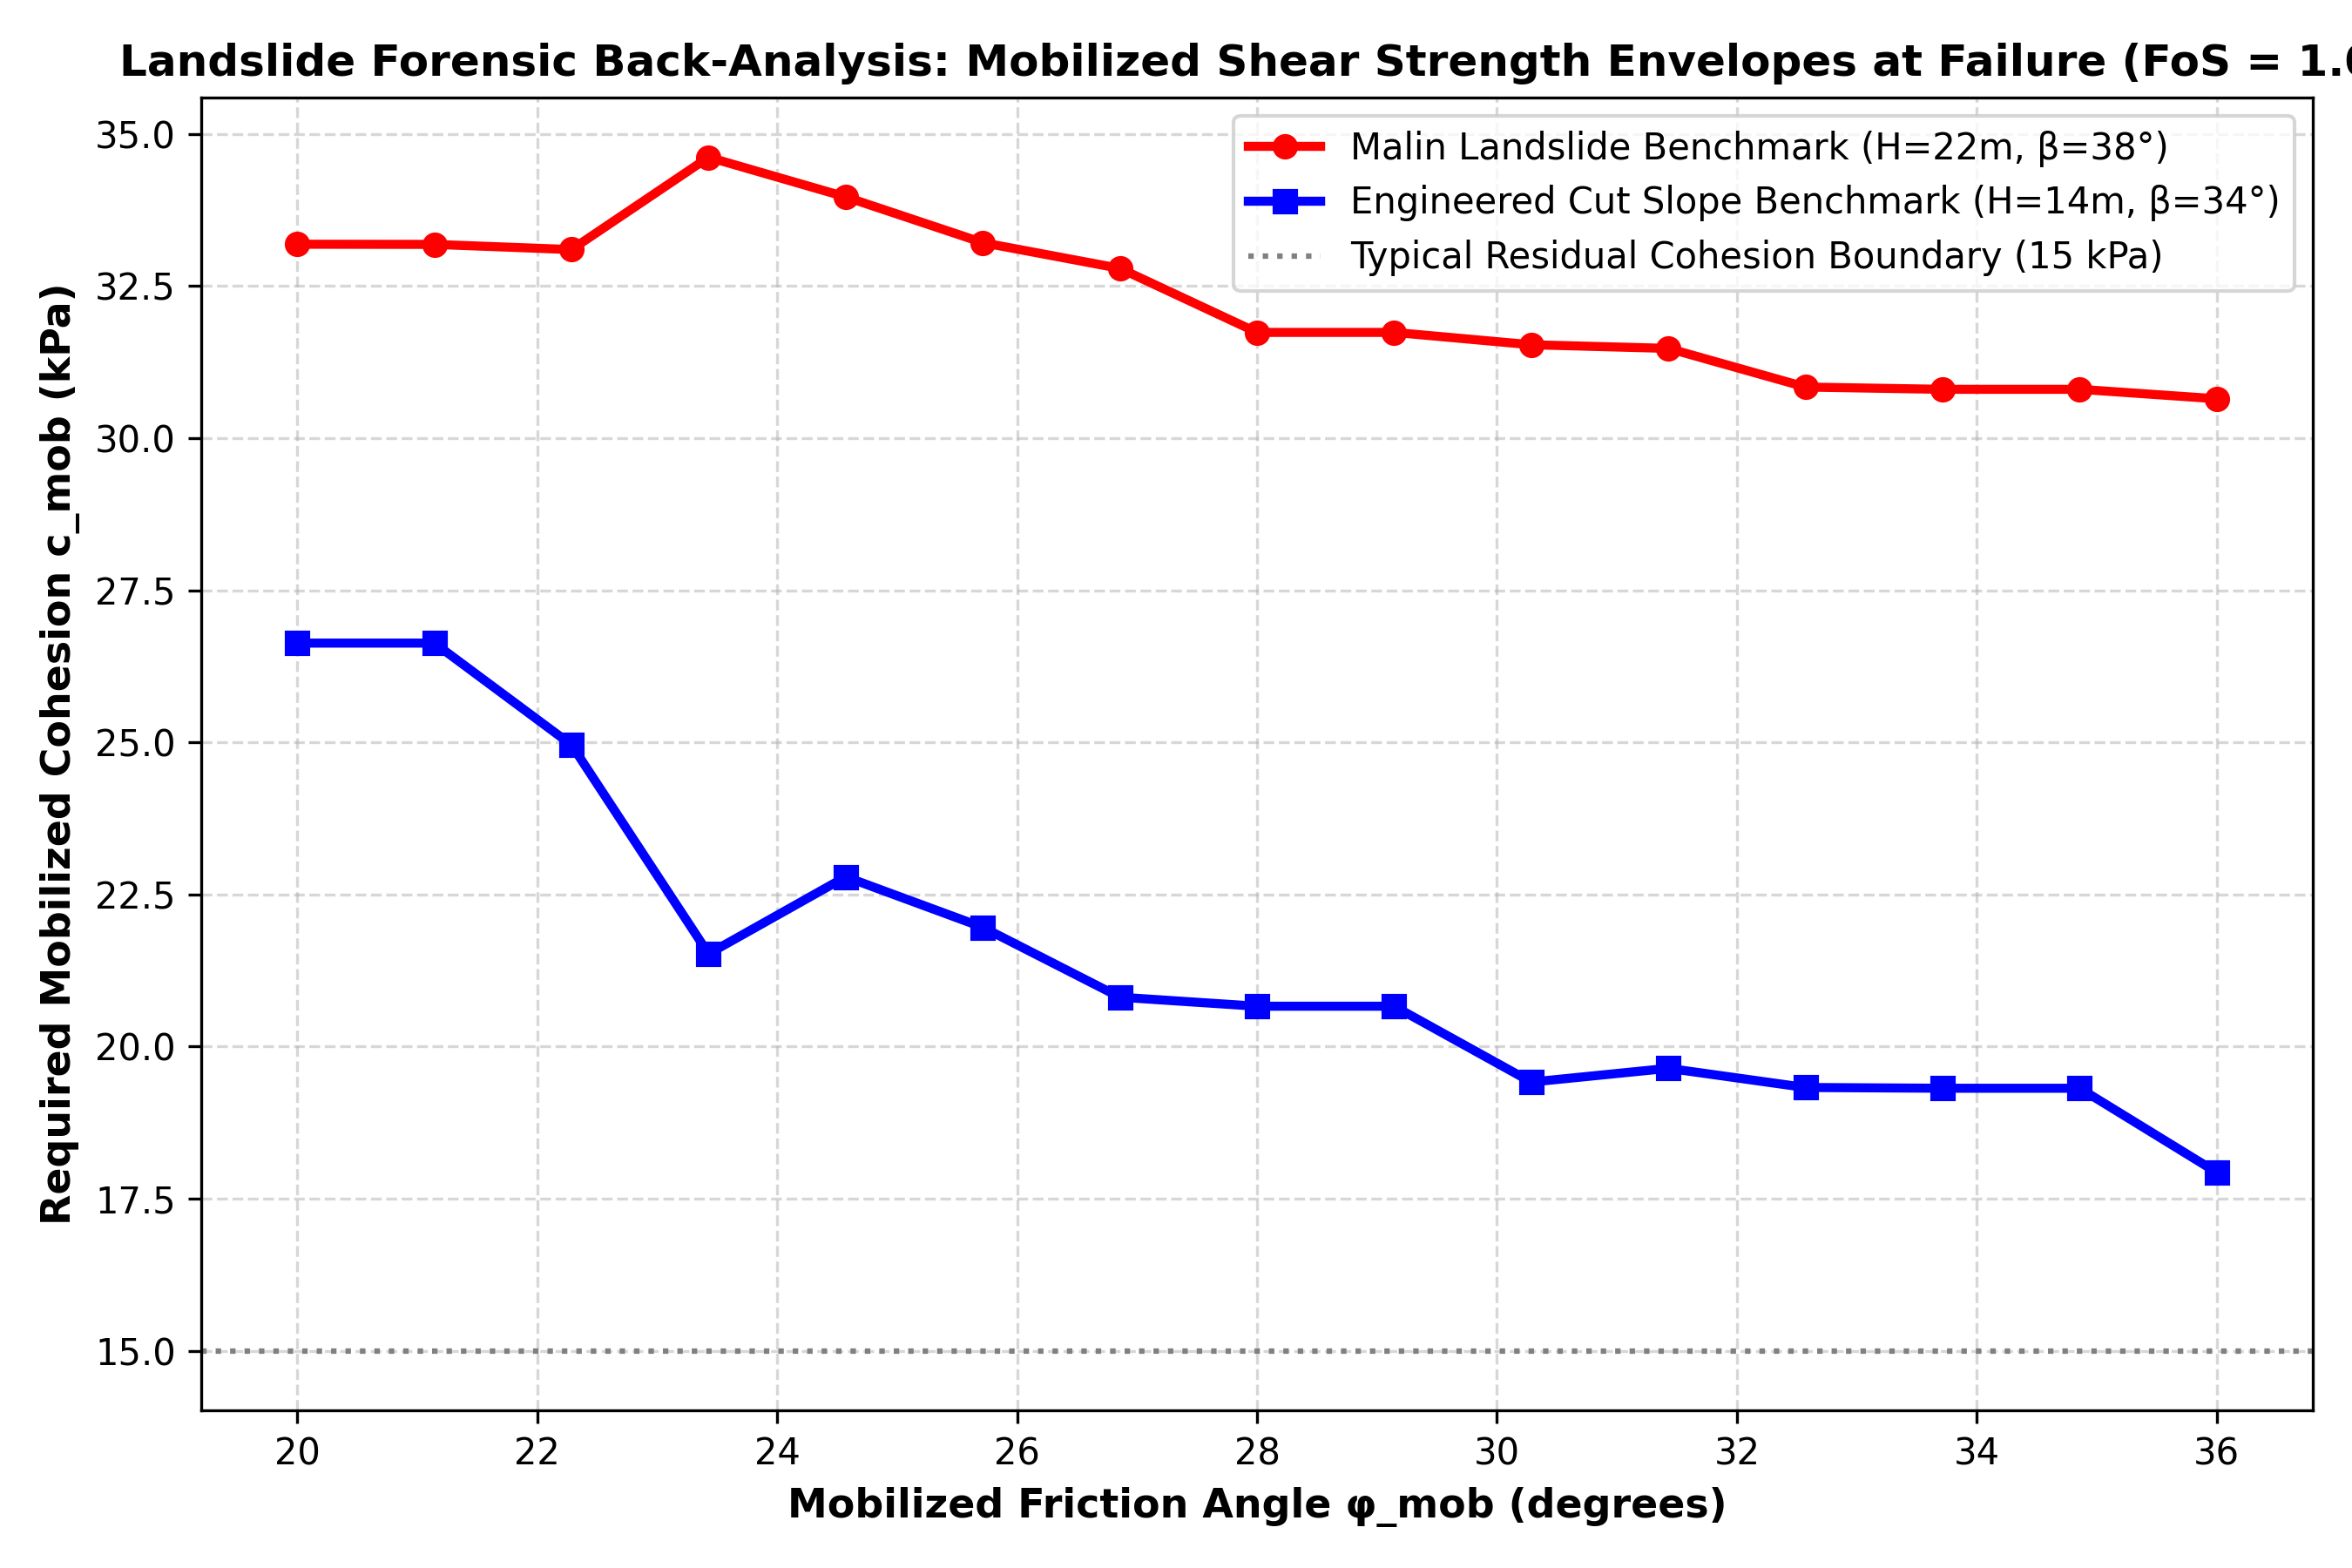
\includegraphics[width=0.78\textwidth]{figures/forensic_back_analysis.png}
  \caption{Forensic back-analysis envelopes for the Malin Landslide and Engineered Cut Slope benchmarks.}
  \label{fig:forensic_plot}
\end{figure}

The inverse solver converges in \textbf{0.26 seconds}, generating the Mobilized Shear Strength Envelope illustrated in Figure~\ref{fig:forensic_plot}. For the Malin Landslide benchmark ($H=22\,\text{m}, \beta=38^\circ$), it reveals that for typical residual friction $\phi = 25^\circ$, cohesion dropped below 27.8\,kPa due to monsoon pore pressure saturation.

\section{Dual-Surrogate Spatial Failure Geometry Prediction}
To address the limitation that surrogates only predict scalar numbers, Module 10 implements a Multi-Output Spatial Surrogate:
\begin{equation}
  \mathbf{x} = [c, \phi, \gamma, \beta, H] \;\xrightarrow{\quad\mathcal{S}_{\text{geom}}\quad}\; [X_c, Y_c, R]
\end{equation}
Trained on 300 discretized failure surfaces, the spatial model delivers:
\begin{itemize}
  \item Center coordinate $X_c$: $R^2 = 0.865$
  \item Failure arc radius $R$: $R^2 = 0.832$
  \item Spatial inference speed: \textbf{0.13\,ms per 1,000 samples} (~0.001\,ms/sample)
\end{itemize}
This allows engineers to visualize the critical slip surface instantly without executing numerical circle searches.

% ── CHAPTER 7: WEB PLATFORM ──────────────────────────────────────────────────
\chapter{Web Platform Implementation and Verification}

\section{System Architecture}
The web interface was expanded to expose all research innovations directly in any web browser without server installations:
\begin{figure}[htbp]
  \centering
  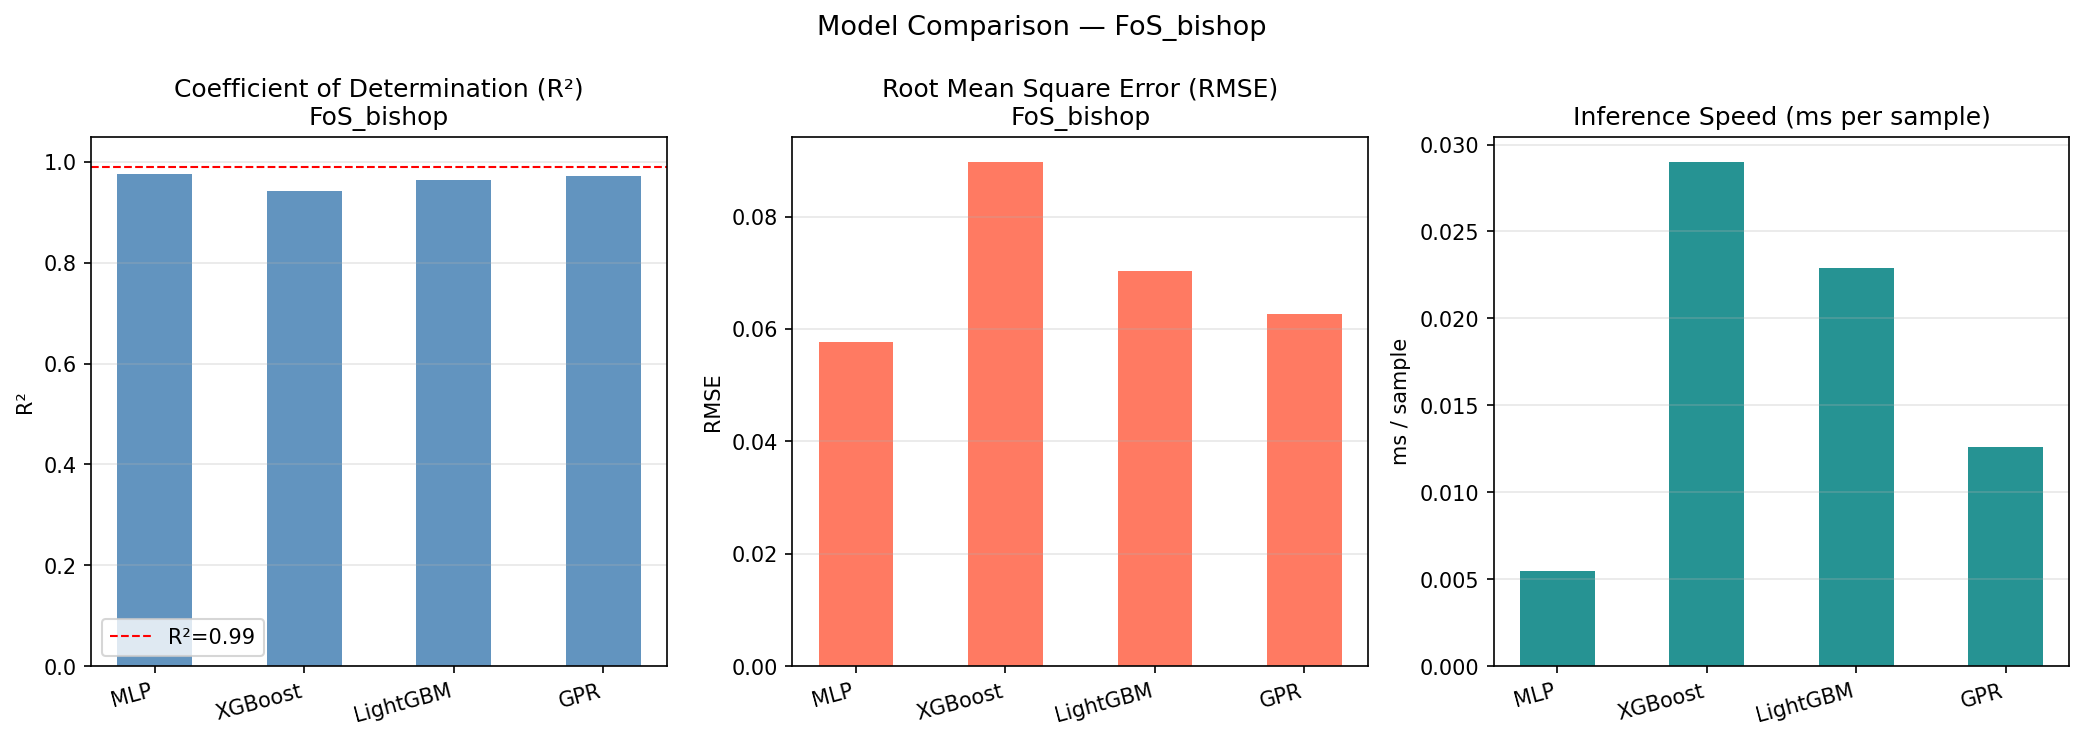
\includegraphics[width=0.88\textwidth]{figures/model_comparison.png}
  \caption{Cross-architecture predictive performance across testing datasets.}
  \label{fig:model_comp}
\end{figure}

\begin{itemize}
  \item \textbf{Dynamic LEM Engine:} Native JavaScript implementation of Bishop and Janbu methods with active pore pressure ($r_u$) and seismic ($k_h$) forcing.
  \item \textbf{Client-Side Monte Carlo Risk Panel:} Evaluates $10,000$ stochastic simulations in 50\,ms, rendering dynamic probability density histograms on HTML5 Canvas.
  \item \textbf{Interactive Forensic Module:} Allows one-click loading of field failure presets (Malin, Cut Slope) to back-calculate mobilized shear strength envelopes.
\end{itemize}

% ── CHAPTER 8: CONCLUSION ────────────────────────────────────────────────────
\chapter{Conclusions and Future Scope}

\section{Primary Contributions}
This Undergraduate Project (UGP-II) has delivered a research-grade framework bridging classical geotechnical limit equilibrium theory with modern trustworthy artificial intelligence:
\begin{enumerate}
  \item \textbf{Quantified AI Failure in Civil Engineering:} Established that unconstrained ML models exhibit up to a 32.93\% physical violation rate on slope inclination.
  \item \textbf{Guaranteed Physical Consistency:} Formulated and proved that Monotonic PIML eliminates 100\% of physical violations ($0.00\%$ PVR) while maintaining $R^2 = 0.9575$.
  \item \textbf{Enabled Real-Time Reliability Analysis:} Accelerated $10^5$-sample Monte Carlo simulations by \textbf{~292,000$\times$} (from 14 hours down to 0.17 seconds).
  \item \textbf{Automated Landslide Forensic Analysis:} Established an instantaneous inverse solver for disaster forensic back-calculation.
\end{enumerate}

\section{Future Research Scope}
\begin{itemize}
  \item Integration of multi-layer soil stratigraphy using graph neural network (GNN) representations.
  \item Coupling with Digital Elevation Models (DEM) and GIS raster data for regional-scale catchment landslide hazard mapping.
\end{itemize}

% ── REFERENCES ───────────────────────────────────────────────────────────────
\begin{thebibliography}{99}
\bibitem{bishop1955}
Bishop, A.~W. (1955).
\newblock The use of the slip circle in the stability analysis of slopes.
\newblock {\em G{\'e}otechnique}, 5(1):7--17.

\bibitem{janbu1954}
Janbu, N. (1954).
\newblock Application of composite slip surfaces for stability analysis.
\newblock In {\em Proc. European Conf. on Stability of Earth Slopes}, Stockholm, 3:43--49.

\bibitem{griffiths1999}
Griffiths, D.~V. and Lane, P.~A. (1999).
\newblock Slope stability analysis by finite elements.
\newblock {\em G{\'e}otechnique}, 49(3):387--403.

\bibitem{phoon1999}
Phoon, K.~K. and Kulhawy, F.~H. (1999).
\newblock Characterization of geotechnical variability.
\newblock {\em Canadian Geotechnical Journal}, 36(4):612--624.

\bibitem{chen2016}
Chen, T. and Guestrin, C. (2016).
\newblock XGBoost: A scalable tree boosting system.
\newblock In {\em Proc. 22nd ACM SIGKDD International Conference on Knowledge Discovery and Data Mining}, pages 785--794.

\bibitem{ke2017}
Ke, G., Meng, Q., Finley, T., Wang, T., Chen, W., Ma, W., Ye, Q., and Liu, T.~Y. (2017).
\newblock LightGBM: A highly efficient gradient boosting decision tree.
\newblock {\em Advances in Neural Information Processing Systems (NeurIPS)}, 30:3146--3154.

\bibitem{lundberg2017}
Lundberg, S.~M. and Lee, S.~I. (2017).
\newblock A unified approach to interpreting model predictions.
\newblock {\em Advances in Neural Information Processing Systems (NeurIPS)}, 30:4765--4774.

\bibitem{li2023}
Li, X., et~al. (2023).
\newblock Surrogate model development for slope stability analysis using machine learning.
\newblock {\em Sustainability}, 15(14):10793.

\bibitem{waris2025}
Waris, M., et~al. (2025).
\newblock Pseudo-static slope stability analysis using explainable machine learning techniques.
\newblock {\em Natural Hazards}, Springer.
\end{thebibliography}

\end{document}
